\documentclass[11pt,spanish]{article} % Tipo y tamaño de letra del documento.

\input{preamble.tex} 

\newcommand{\tnum}{2 y 3} % reemplace 2 por el número de la tarea
\newcommand{\sem}{2024-2} % reemplace 2024-2 por el semestre correspondiente
\newcommand{\campus}{San Joaquin\\ Santiago} % reemplace Casa Central por el campus correspondiente
\newcommand{\rolusm}{202004556-9} % reemplace 2025073100-1 por su rol
\newcommand{\namestudent}{Francisco Rebolledo C.} % reemplace Al Goritmo Pérez por su nombre

\headheight=14pt
\linespread{1.3}
\author{\namestudent}
\pagestyle{fancy}
\fancyhf{}%
\fancyfoot[R]{ \namestudent \\ \rolusm}
\fancyfoot[L]{Campus \campus} 
\fancyfoot[C]{\thepage}
\rhead{2024-2}
\lhead{INF-221}
\renewcommand{\headrulewidth}{0.4pt}
\renewcommand{\footrulewidth}{0.4pt}
\newbool{programs}
\boolfalse{programs}
\chead{REPORTE TAREA \tnum~}



\title{
  \huge
  \textbf{REPORTE TAREA \tnum~ \\ ALGORITMOS Y COMPLEJIDAD} \\[1ex]
  \emph{\textquote{Explorando la Distancia entre Cadenas, una Operación a la Vez}}
  }

  
\date{
  \small
  \today\\
  \currenttime
}




\begin{document}
\maketitle
\thispagestyle{fancy} 
\vspace{-1.0\baselineskip}




\begin{abstract}
  \textit{ 
    En este reporte se presenta un análisis de algoritmos sobre el problema de la distancia mínima de edición, haciendo especial énfasis en la diferencia de la complejidad temporal y en memoria que pueden presentar los enfoques de Fuerza Bruta y Programación Dinámica dentro de un mismo problema, esto mediante la directa implementación de dichos enfoques en una infraestructura de programas que abordan distintos tipos de casos con la misión de obtener los resultados de la forma más precisa y limpia posible para comprobar de forma práctica la importancia que tiene el análisis y diseño de algoritmos en la resolución de problema complejos mediante las ciencias de la computación y como la forma de dar solución a un problema mediante distintos enfoques de algoritmo puede cambiar su complejidad.

  }
     
\end{abstract}

\setcounter{tocdepth}{1}
\tableofcontents


\newpage
\section{Introducción}
Hace años que la computación es una de las mejores herramientas para la resolución de problemas en diversas áreas debido a que nos permite procesar grandes volúmenes de datos rápidamente, automatizar tareas y encontrar soluciones optimas que manualmente resultaría imposible. Dentro de las ciencias de la computación una de las ramas mas importantes es el \textbf{Análisis y Diseño de Algoritmos}, ya que permite desarrollar métodos eficientes para resolver problemas complejos.\\

Este trabajo se enfoca en comparar estos dos enfoques, considerando su complejidad temporal y espacial, y analizando cómo la naturaleza del problema y las características de las cadenas de entrada, como su simetría o asimetría, afectan el rendimiento de los algoritmos. El análisis de estos dos enfoques no solo proporciona una visión clara sobre sus diferencias fundamentales, sino también sobre cómo cada uno se comporta al enfrentar el problema bajo distintas condiciones y restricciones.

\newpage
\section{Diseño y Análisis de Algoritmos} 
El problema de la \textbf{Distancia Mínima de Edición} tiene varias formas de ser abordado, las cuales pueden tener una gran diferencia en la eficiencia de la memoria o los tiempos de ejecución de los algoritmos. Por lo mismo, antes de entrar directamente en el análisis de los algoritmos resulta importante definir el diseño que seguirán los paradigmas para tener en cuenta cuáles son sus principales diferencias y como esto puede llegar a afectar a la solución que dan al problema.\\

En general, estos enfoques buscaran abordar el problema una letra a la vez pero se separan de tal forma que, por \textbf{Fuerza Bruta} el algoritmo deberá calcular y almacenar cada una de las 4 operaciones fundamentales (insertar, borrar, reemplazar y transponer) por cada letra, creando un crecimiento exponencial al buscar cada combinación probable, mientras que el algoritmo con enfoque de \textbf{Programación Dinámica} identificará y almacenará los costos de edición de cadenas mas cortas dentro de la cadena principal para armar en base a estas el costo de la cadena principal.\\

Además, también resulta importante analizar la naturaleza del problema, pues el hecho de que cada operación tenga \textbf{costos variables} en base al o los caracteres involucrados agrega una capa de complejidad a los algoritmos que deben trabajar para decidir qué operación es la más adecuada en cada caso, lo que puede aumentar el tiempo de ejecución de los mismos dadas las operaciones necesarias para el procedimiento. Por lo mismo, agregar la \textbf{operación de transposición} aumenta las posibilidades de los caminos a tomar y variables que tener en cuenta, lo que incrementa aun más la complejidad del problema pero especialmente representa una carga en el enfoque de Fuerza Bruta al considerar exhaustivamente todas las formas de modificar la cadena.\\
\newpage

\subsection{Fuerza Bruta}


\subsubsection{Descripción de la solución}

El algoritmo diseñado funciona de forma recursiva para abordar una cantidad mayor de casos sin colapsar la memoria del computador pero sin abandonar el principio de fuerza bruta al buscar exhaustivamente entre todas las posibilidades generadas en el árbol recursivo, la base del algoritmo es ir letra por letra evaluando las 4 operaciones y repetir por cada una para la letra siguiente hasta llegar a transformar la cadena1 en la cadena2 y luego buscar cual tuvo el mínimo costo.

\subsubsection{Complejidad Temporal y Espacial}

Dada la forma del problema, las complejidades están directamente relacionadas al largo de las cadenas, por lo que \textbf{a} y \textbf{b} son respectivamente el número de caracteres para cadena1 y cadena2. Definidos estos valores, \textbf{n} representa todos los posibles valores, por lo que se asume que sera la cadena más larga. Para el análisis de la complejidad temporal y espacial, se verifica que la función posee un factor de recurrencia de 4 y va guardando todos los posibles valores, por lo que se obtienen los valores:
\begin{center}
\begin{tabular}{c|c}
\textbf{Complejidad Temporal} & \textbf{Complejidad Espacial} \\ \hline
$T(n) = O(4^{ n})$ & $E(n) = O(n))$
\end{tabular}
\end{center}

\subsubsection{Pseudocódigo del algoritmo utilizando fuerza bruta}

\begin{algorithm}[H]
\DontPrintSemicolon
\KwFunction{$\textbf{Procedure}\text{ DME\_Fuerza\_Bruta}(\text{cadena1}, \text{cadena2}, i, j)$}\\
    \If{$i == 0$}{
        \Return $j \cdot \text{costo\_ins}(\text{cadena2}[j-1])$\;
    }
    \If{$j == 0$}{
        \Return $i \cdot \text{costo\_del}(\text{cadena1}[i-1])$\;
    }
    
    \If{$\text{cadena1}[i-1] == \text{cadena2}[j-1]$}{
        \Return $\text{DME\_Fuerza\_Bruta}(\text{cadena1}, \text{cadena2}, i-1, j-1)$\;
    }
    
    $insertar \gets \text{DME\_Fuerza\_Bruta}(\text{cadena1}, \text{cadena2}, i, j-1) + \text{costo\_ins}(\text{cadena2}[j-1])$\;
    $eliminar \gets \text{DME\_Fuerza\_Bruta}(\text{cadena1}, \text{cadena2}, i-1, j) + \text{costo\_del}(\text{cadena1}[i-1])$\;
    $sustituir \gets \text{DME\_Fuerza\_Bruta}(\text{cadena1}, \text{cadena2}, i-1, j-1) + \text{costo\_sub}(\text{cadena1}[i-1], \text{cadena2}[j-1])$\;
    
    $transponer \gets \infty$\;
    \If{$i > 1$ \KwAnd $j > 1$ \KwAnd $\text{cadena1}[i-1] == \text{cadena2}[j-2]$ \KwAnd $\text{cadena1}[i-2] == \text{cadena2}[j-1]$}{
        $transponer \gets \text{DME\_Fuerza\_Bruta}(\text{cadena1}, \text{cadena2}, i-2, j-2) + \text{costo\_trans}(\text{cadena1}[i-2], \text{cadena1}[i-1])$\;
    }
    
    \Return $\min(\{insertar, eliminar, sustituir, transponer\})$\;
\caption{DME\_Fuerza\_Bruta}
\end{algorithm}
\subsection{Programación Dinámica}
\subsubsection{Descripción de la solución}

De forma similar, pero con mucha menor complejidad en comparación al enfoque de fuerza bruta, la solución al problema se encuentra al plantear la recursividad de la función principal, con la diferencia esta vez de que se deben guardar los casos intermedios para utilizarlos en la construcción de la solución principal. Por lo que primero, el algoritmo construye una matriz de tamaño (a+1)×(b+1), donde a y b son las longitudes de las cadenas A y B respectivamente, con el motivo de almacenar los costos mínimos de transformar los primeros i caracteres de una cadena en los primeros j de la otra. Luego, inicializa los casos base para manejar transformaciones desde o hacia cadenas vacías y después llena la matriz evaluando las operaciones de insertar, eliminar, reemplazar y, si es posible, transponer caracteres. Así, el costo mínimo para cada operación se calcula de forma acumulativa, evitando cálculos redundantes. Finalmente, el valor en la celda (a,b) de la matriz representa el costo mínimo total.

\subsubsection{Relación de recurrencia}

\begin{equation*}
    matriz[i][j] = \min \begin{cases}
    matriz[i-1][j] + \text{costo de eliminación} \\
    matriz[i][j-1] + \text{costo de inserción} \\
    matriz[i-1][j-1] + \text{costo de sustitución}  \\
    matriz[i-2][j-2] + \text{costo de transposición}
    \end{cases}
\end{equation*}


\subsubsection{Identificación de subproblemas}

Los subproblemas son las distancias mínimas de edición entre todos los prefijos de las dos cadenas. Específicamente, los subproblemas corresponden a calcular la distancia mínima de edición entre los primeros i caracteres de la primera cadena y los primeros j caracteres de la segunda cadena. La solución final se obtiene calculando la distancia entre las cadenas completas, es decir, entre los primeros a caracteres de la primera cadena y los primeros b caracteres de la segunda cadena.

\subsubsection{Complejidad Temporal y Espacial}

Para obtener las complejidades con un enfoque de programación dinámica resulta relevante el largo de las 2 cadenas para el tamaño de la matriz de memoria que se creará en el proceso, como se menciono anteriormente, a es la longitud de la primera cadena y b es la longitud de la segunda cadena. Con esto, el algoritmo llena una matriz de dimensiones (a+1)×(b+1), calculando cada celda de la matriz en tiempo constante y de forma que cada celda almacena un subproblema. Bajo esta descripción se puede verificar:

\begin{center}
\begin{tabular}{c|c}
\textbf{Complejidad Temporal} & \textbf{Complejidad Espacial} \\ \hline
$T(n) = O(a * b) = O(n^{2})$ & $E(n) = O(a * b) =  O(n^{2})$
\end{tabular}
\end{center}

\subsubsection{Algoritmo utilizando programación dinámica}

\begin{algorithm}[H]
\DontPrintSemicolon
\KwFunction{$\textbf{Procedure}\text{ DME\_Programacion\_Dinamica}(\text{cadena1}, \text{cadena2})$}\\
    $a \gets \text{len}(\text{cadena1})$\;
    $b \gets \text{len}(\text{cadena2})$\;
    
    Crear matriz $matriz$ de tamaño $(a+1) \times (b+1)$ inicializada con ceros\;
    
    \For{$i \gets 0$ \KwTo $a$}{
        $matriz[i][0] \gets i \cdot \text{costo\_del}(\text{cadena1}[i-1])$\;
    }
    \For{$j \gets 0$ \KwTo $b$}{
        $matriz[0][j] \gets j \cdot \text{costo\_ins}(\text{cadena2}[j-1])$\;
    }
    
    \For{$i \gets 1$ \KwTo $a$}{
        \For{$j \gets 1$ \KwTo $b$}{
            \If{$\text{cadena1}[i-1] == \text{cadena2}[j-1]$}{
                $matriz[i][j] \gets matriz[i-1][j-1]$\;
            }
            \Else{
                $matriz[i][j] \gets \min\Big($ \;
                \Indp
                $matriz[i-1][j] + \text{costo\_del}(\text{cadena1}[i-1]),$ \;
                $matriz[i][j-1] + \text{costo\_ins}(\text{cadena2}[j-1]),$ \;
                $matriz[i-1][j-1] + \text{costo\_sub}(\text{cadena1}[i-1], \text{cadena2}[j-1])$ \;
                \Indm
                $\Big)$\;
            }
            
            \If{$i > 1$ \KwAnd $j > 1$ \KwAnd $\text{cadena1}[i-1] == \text{cadena2}[j-2]$ \KwAnd $\text{cadena1}[i-2] == \text{cadena2}[j-1]$}{
                $matriz[i][j] \gets \min\Big($\;
                \Indp
                $matriz[i][j],$ \;
                $matriz[i-2][j-2] + \text{costo\_trans}(\text{cadena1}[i-1], \text{cadena1}[i-2])$\;
                \Indm
                $\Big)$\;
            }
        }
    }
    \Return $matriz[a][b]$\;
\caption{DME\_Programacion\_Dinamica}
\end{algorithm}
\newpage
\section{Implementaciones}
Todos los códigos y dependencias utilizados se encuentran en el siguiente enlace de Github, además, las instrucciones para trabajar con los programas deben realizarse en dicho directorio por consola.

\begin{mdframed}
\url{https://github.com/sPyKeRT1/FranciscoRebolledo_Tarea2_3/tree/main/codigos}
\end{mdframed}

Para trabajar de mejor forma los programas de C++ y facilitar su uso junto al generador de casos de prueba en Python se utiliza la herramienta Makefile bajo las siguientes instrucciones:

\begin{itemize}
    \item \textbf{make create}: Inicia Generador.py para crear el caso de prueba con ciertos parámetros.
    \item \textbf{make all}: Compila los archivos de C++ para posteriormente ejecutarlos junto a los demás.
    \item \textbf{make run}: Ejecuta los programas en el orden Programación Dinámica->Fuerza Bruta.
    \item \textbf{make clear}: Elimina los archivos objetivo necesarios para ejecutar los programas de C++.
\end{itemize}

La estructura general que da soporte para implementar las funcionalidades esperadas para los algoritmos consta de 5 archivos de texto para guardar por separado las palabras en \textbf{'cadenas.txt'} y las 4 tablas de costos para las operaciones insertar en \textbf{'cost\_insert.txt'}, borrar en \textbf{'cost\_delete.txt'}, reemplazar en \textbf{'cost\_replace.txt'} y transponer en \textbf{'cost\_transpose.txt'}; además, se implementa \textbf{'generador.py'} para crear un caso de prueba en base a los parámetros que se le entreguen por entrada estándar y junto a esto, se agregan los archivos \textbf{'funcostos.h'} y \textbf{'funcostos.cpp'} donde se definen e implementan las funciones que obtienen los costos directamente desde las tablas antes mencionadas para los algoritmos.\\

Al implementar los algoritmos en \textbf{'progfuerzabruta.cpp'} y \textbf{'progdinamica.cpp'} se busca mantener los algoritmos lo más limpios posible para que no deban realizar tareas de entrada o salida de datos fuera del llamado a las funciones de costo, por lo que, primero leen desde el archivo 'cadenas.txt' las cadenas de caracteres a trabajar y las pasan como parámetro a las funciones \textbf{DME\_Fuerza\_Bruta(cadena1, cadena2, tamaño\_cadena1, tamaño\_cadena2)} y \textbf{DME\_Programacion\_Dinamica(cadena1, cadena2)}  de forma respectiva, las cuales como se mostró anteriormente ejecutan el algoritmo 
correspondiente y devuelven la distancia mínima de edición para que después la función main se encargue de mostrar los datos obtenidos del proceso por pantalla y finalizar su ejecución. 


\newpage
\section{Experimentos}

Para la replicación de este experimento es crucial la reproducibilidad de los resultados por lo que a continuación se detallan las especificaciones del equipo utilizado a nivel de hardware y software:

\begin{itemize}
    \item Procesador: Intel(R) Core(TM) i5-10300H CPU @ 2.50GHz 2.50 GHz
    \item RAM: 16,0 GB DDR4
    \item Almacenamiento: SK hynix BC511 HFM512GDJTNI-82A0A (SSD)
    \item Sistema Operativo: Edición Windows 10 Home Single Language, Versión	22H2, Compilación del SO 19045.5131, Experiencia Windows Feature Experience Pack 1000.19060.1000.0
    \item Compilador: g++.exe (Rev3, Built by MSYS2 project) 14.1.0
\end{itemize}
\subsection{Dataset (casos de prueba)}
Para verificar y probar correctamente la funcionalidad de los algoritmos ya sea de Fuerza Bruta o Programación Dinámica aparte de usar los casos aleatorios con crecimiento en el número de caracteres es importante obtener resultados con casos que posean ciertas características distintivas o limites respecto a los demás, es por ello que los 5 principales serán casos con cadenas de caracteres vacíos, cadenas de caracteres repetidos, cadenas simétricas, cadenas asimétricas y donde las matrices tienen un mismo valor para todas las operaciones, casos los cuales tienen al rededor de 5 caracteres por cadena para que esta variable no afecte en los resultados. (Estos datasets pueden ser encontrados en sus respectivas carpetas dentro del repositorio de Github o como imágenes en el apéndice de este reporte)\\

1. \underline{Caso con cadenas vacías:} En este \hyperref[fig:imagen1]{caso} se deben testear cadenas sin ningún carácter para ver el funcionamiento correcto de los algoritmos y ver cual posee mayor efectividad al lidiar con tal problemática.\\

2. \underline{Caso con caracteres repetidas:} La característica de este \hyperref[fig:imagen2]{caso} es que las cadenas son repeticiones de un mismo carácter para ver si la repetición de un subproblema hace al algoritmo más eficiente.\\

3. \underline{Caso con cadenas simétricas:} La intención de este \hyperref[fig:imagen3]{caso} es ver si ayuda de alguna forma a los algoritmos que las cadenas posean igual cantidad de caracteres y compararlo con las cadenas asimétricas.\\

4. \underline{Caso con cadenas asimétricas:} Este \hyperref[fig:imagen4]{caso} va de la mano con el anterior y sirve para verificar si las cadenas de distinto largo tienen algún impacto en los tiempos de ejecución y la respuesta de los algoritmos.\\

5. \underline{Caso con matrices con valores iguales:} Por último \hyperref[fig:imagen5]{caso}, resulta interesante verificar el efecto de matrices iguales o planas en sus valores y como esto puede afectar en la calidad de sus respuestas.\\


\subsection{Resultados}
Primero y siguiendo con el orden de los datasets mostrados serán presentados los resultados referentes a los casos limite y luego como aumentan respecto al aumento de caracteres de forma simétrica:\\

1. Caso con cadenas vacías: \\
\begin{figure}[ht]
  \centering
  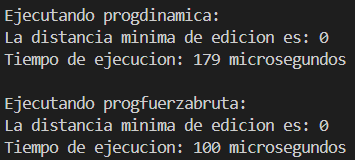
\includegraphics[width=0.6\textwidth]{./images/Resultados1.png}
  \caption{Resultados para el caso limite 1}
  \label{fig:imagen}
\end{figure}

2. Caso con cadenas repetidas:\\
\begin{figure}[ht]
  \centering
  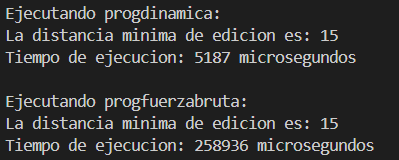
\includegraphics[width=0.6\textwidth]{./images/Resultados2.png}
  \caption{Resultados para el caso limite 2}
  \label{fig:imagen}
\end{figure}

3. Caso con cadenas simétricas:\\
\begin{figure}[ht]
  \centering
  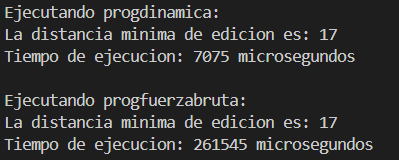
\includegraphics[width=0.6\textwidth]{./images/Resultados3.png}
  \caption{Resultados para el caso limite 3}
  \label{fig:imagen}
\end{figure}
\newpage
4. Caso con cadenas asimétricas:\\
\begin{figure}[ht]
  \centering
  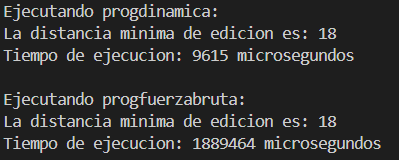
\includegraphics[width=0.6\textwidth]{./images/Resultados4.png}
  \caption{Resultados para el caso limite 4}
  \label{fig:imagen}
\end{figure}

5. Caso con matrices con valores iguales:\\
\begin{figure}[ht]
  \centering
  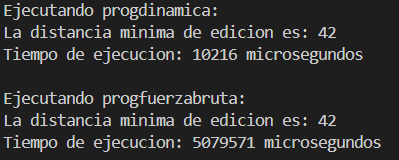
\includegraphics[width=0.6\textwidth]{./images/Resultados5.png}
  \caption{Resultados para el caso limite 5}
  \label{fig:imagen}
\end{figure}

6. Progresión respecto al aumento de caracteres:\\
\begin{figure}[ht]
  \centering
  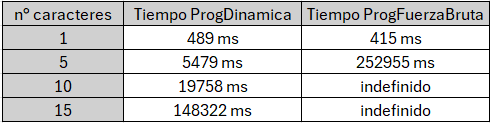
\includegraphics[width=0.6\textwidth]{./images/Resultados6.png}
  \caption{Resultados para la progresión con aumento de caracteres}
  \label{fig:imagen}
\end{figure}
\newpage
\subsection{Analisis de Resultados}

Es posible ver para la Fuerza Bruta que a medida que incrementa el número de caracteres en las cadenas de entrada, la cantidad de llamadas recursivas y los subproblemas a resolver aumenta drásticamente, lo que provoca una crecimiento exponencial del tiempo de ejecución. En experimentos prácticos, se observa que, para cadenas de longitud moderada, el tiempo de ejecución aumenta significativamente, y se vuelve inviable para cadenas más largas (por ejemplo, más de 10-12 caracteres). Esto se debe a que el número de subproblemas crece exponencialmente con el tamaño de las cadenas, lo que hace que el algoritmo sea muy lento.\\

La Programación Dinámica mejora considerablemente la eficiencia del algoritmo, ya que solo resuelve cada subproblema una vez. Este enfoque es significativamente más rápido en comparación con la fuerza bruta, especialmente cuando las cadenas tienen longitudes mayores. Los resultados experimentales muestran que incluso con cadenas de 100 o más caracteres, el algoritmo de Programación Dinámica es mucho más rápido y sigue siendo manejable en términos de tiempo de ejecución.\\

En el caso de cadenas simétricas, el algoritmo de Fuerza Bruta sigue siendo relativamente lento y peor que el de Programación Dinámica, ya que evalúa todas las combinaciones posibles de operaciones. Sin embargo, debido a la regularidad de la estructura de las cadenas, el número de subproblemas realmente distintos a resolver puede ser menor, lo que reduce parcialmente el tiempo de ejecución. Por otro lado, en el caso de cadenas asimétricas, la Fuerza Bruta se ve seriamente afectada. Debido a la falta de regularidad en la estructura de las cadenas, el número de subproblemas a resolver crece de manera exponencial.\\


\newpage
\section{Conclusiones}
En base a los resultados obtenidos, se puede concluir que el \textbf{enfoque de Programación Dinámica ofrece una solución mucho más eficiente al problema de la Distancia Mínima de Edición que el enfoque de Fuerza Bruta}, especialmente cuando se trata de cadenas de caracteres largas. La Fuerza Bruta presenta un crecimiento exponencial en el tiempo de ejecución a medida que se incrementan los caracteres, lo que la convierte en una opción inviable para entradas de mayor tamaño debido a su complejidad. En cambio, la Programación Dinámica optimiza este proceso al dividir el problema en subproblemas más pequeños y reutilizar los resultados previamente calculados, lo que reduce significativamente los tiempos de ejecución y hace que el algoritmo sea escalable.\\

Además, al considerar cadenas simétricas y asimétricas, se observó que la Fuerza Bruta se ve gravemente afectada en el caso de cadenas asimétricas, donde la cantidad de combinaciones posibles de operaciones es mucho mayor. En comparación, el algoritmo de Programación Dinámica se comporta de manera mucho más eficiente independientemente de la simetría de las cadenas, demostrando la robustez de este enfoque. En resumen, la Programación Dinámica es claramente la mejor opción para resolver el problema de la Distancia Mínima de Edición en términos de tiempo y eficiencia, especialmente cuando se manejan cadenas de texto grandes o complejas. En general, se verifica la hipótesis preliminar respecto a como los enfoques pueden cambiar la resolución de un problema y que tan importante es el Diseño y Análisis de Algoritmos para encontrar las soluciones optimas a este.\\

Una posible mejora sería optimizar el uso de memoria mediante la reducción del espacio de almacenamiento necesario. En lugar de utilizar una matriz completa para almacenar los resultados de todos los subproblemas, se podría emplear una estructura de memoria más compacta, como una matriz unidimensional o una técnica de compresión de los resultados intermedios. De todos modos, independiente de los resultados obtenidos se evidencio que existe una falencia en la comprobación de la complejidad espacial, es decir, el uso de memoria lo cual debe ser mejorado y abarcado de mejor forma en posteriores investigaciones.

\newpage

\section{Condiciones de entrega}
\input{condiciones}

\newpage
\appendix


\section{Apéndice 1}
\begin{figure}[ht]
  \centering
  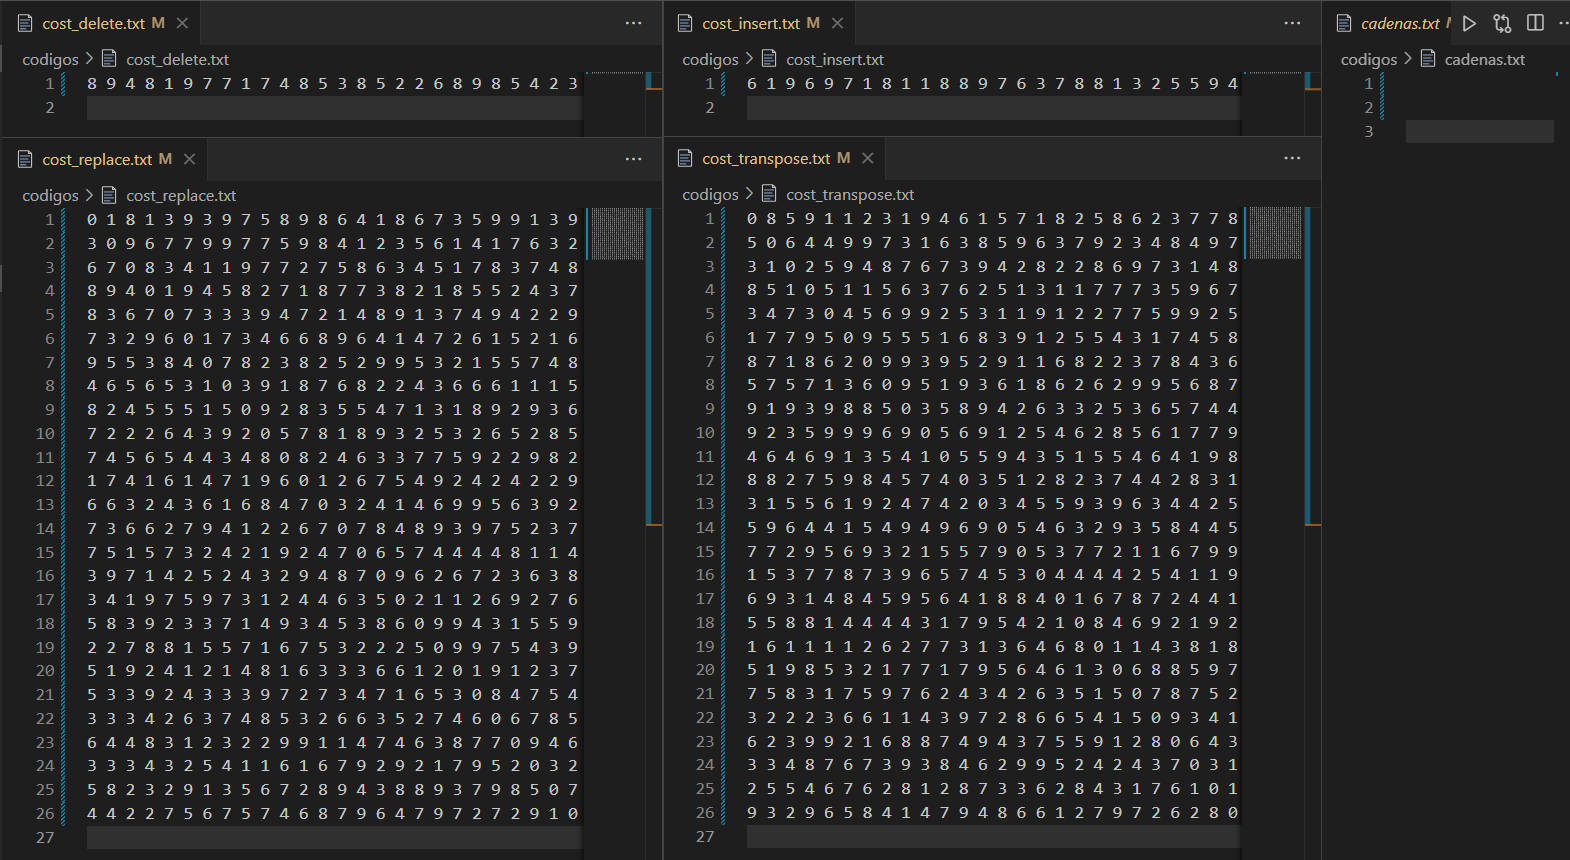
\includegraphics[width=0.8\textwidth]{./images/Casos1.png}
  \caption{Tablas de Costo y Cadenas para el Caso con Cadenas Vacías}
  \label{fig:imagen1}
\end{figure}

\begin{figure}[ht]
  \centering
  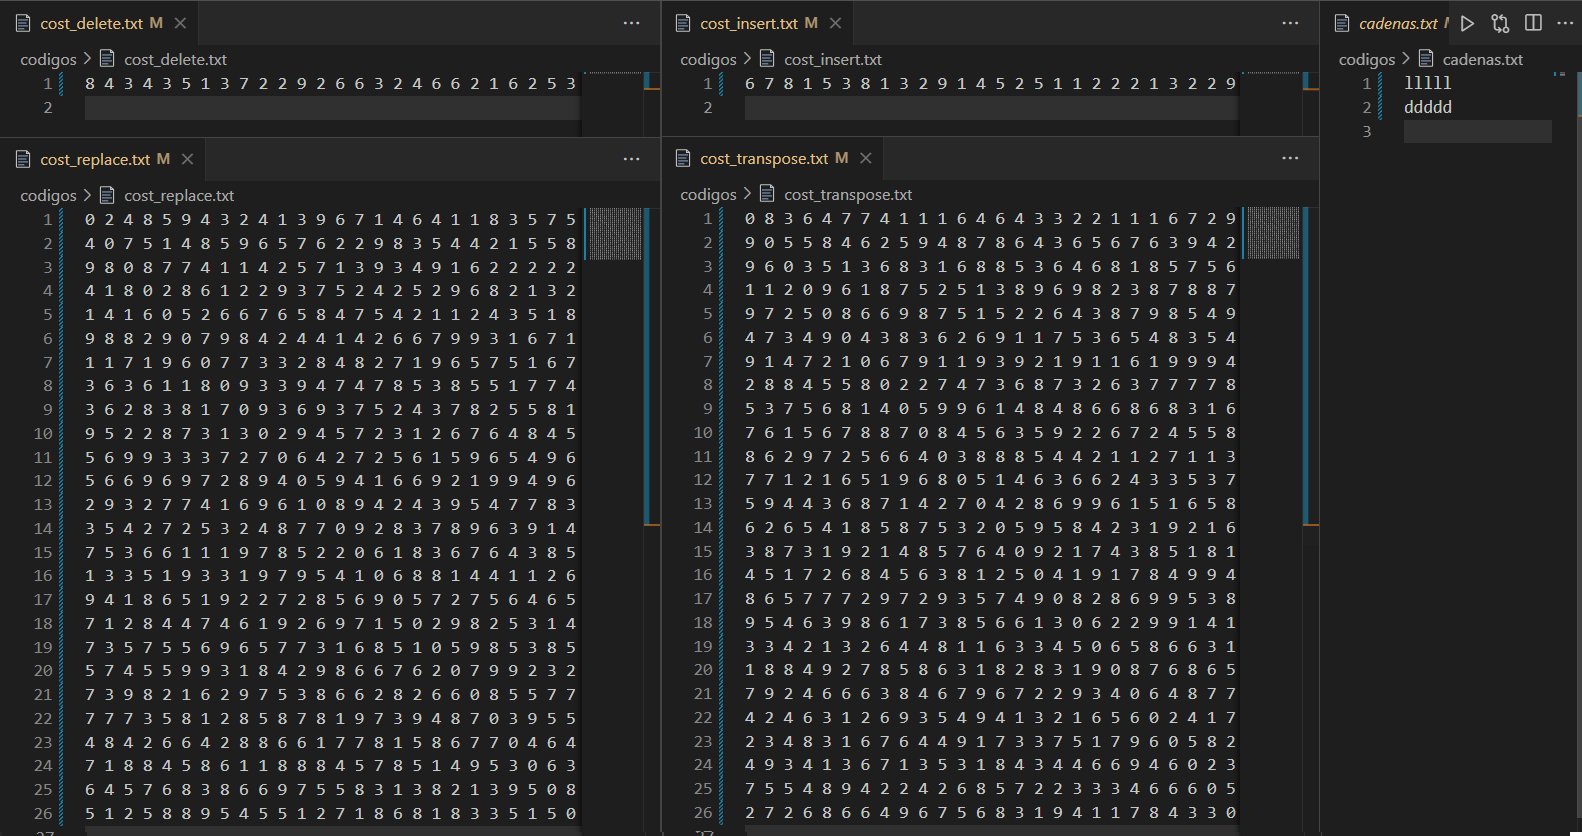
\includegraphics[width=0.8\textwidth]{./images/Casos2.png}
  \caption{Tablas de Costo y Cadenas para el Caso con Caracteres Repetidos}
  \label{fig:imagen2}
\end{figure}

\begin{figure}[ht]
  \centering
  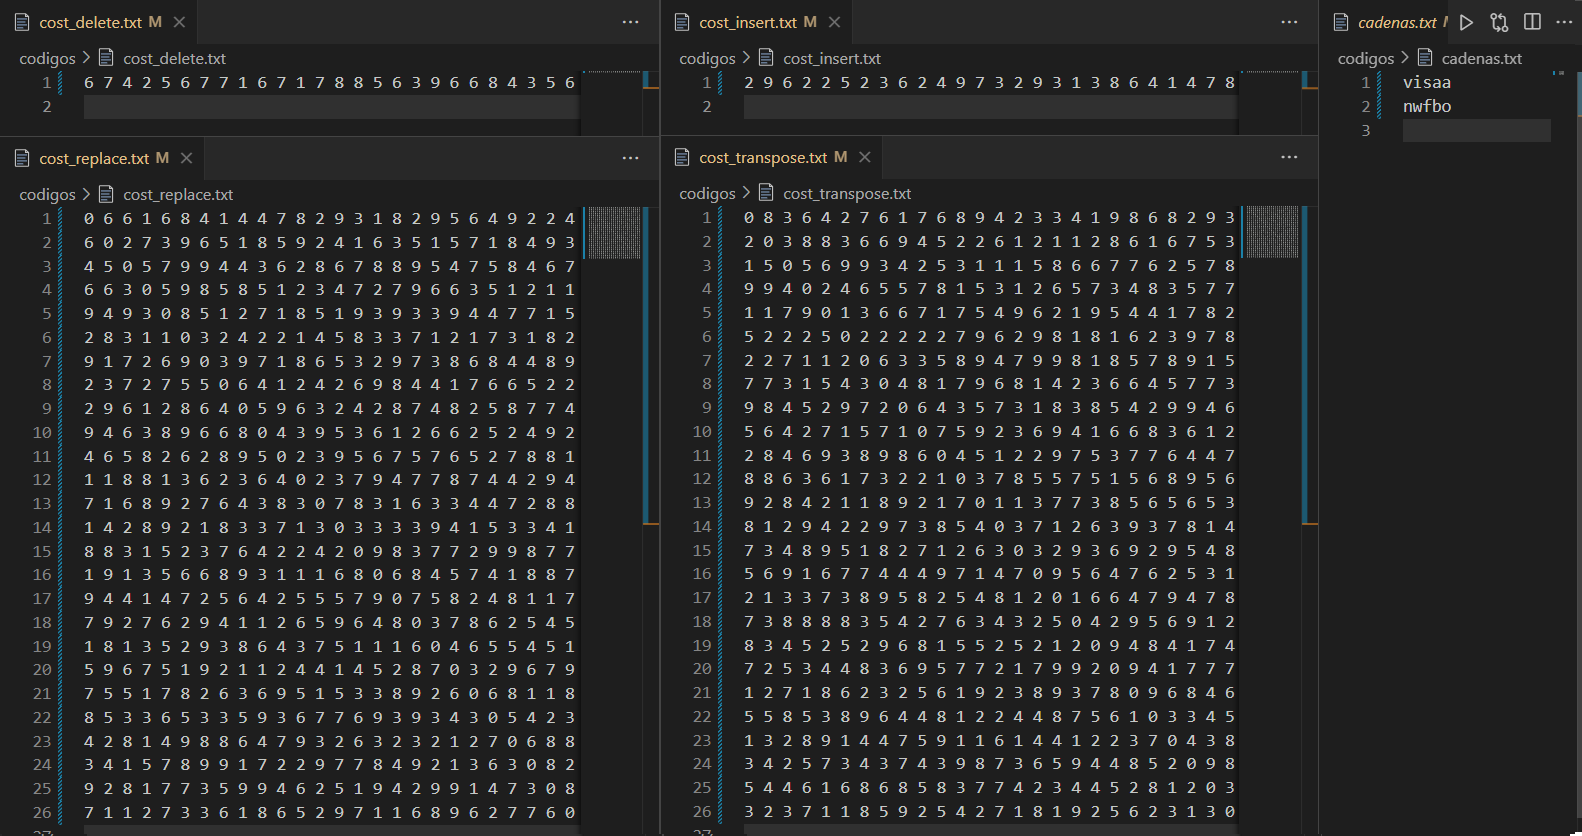
\includegraphics[width=0.6\textwidth]{./images/Casos3.png}
  \caption{Tablas de Costo y Cadenas para el Caso con Cadenas Simétricas}
  \label{fig:imagen3}
\end{figure}

\begin{figure}[ht]
  \centering
  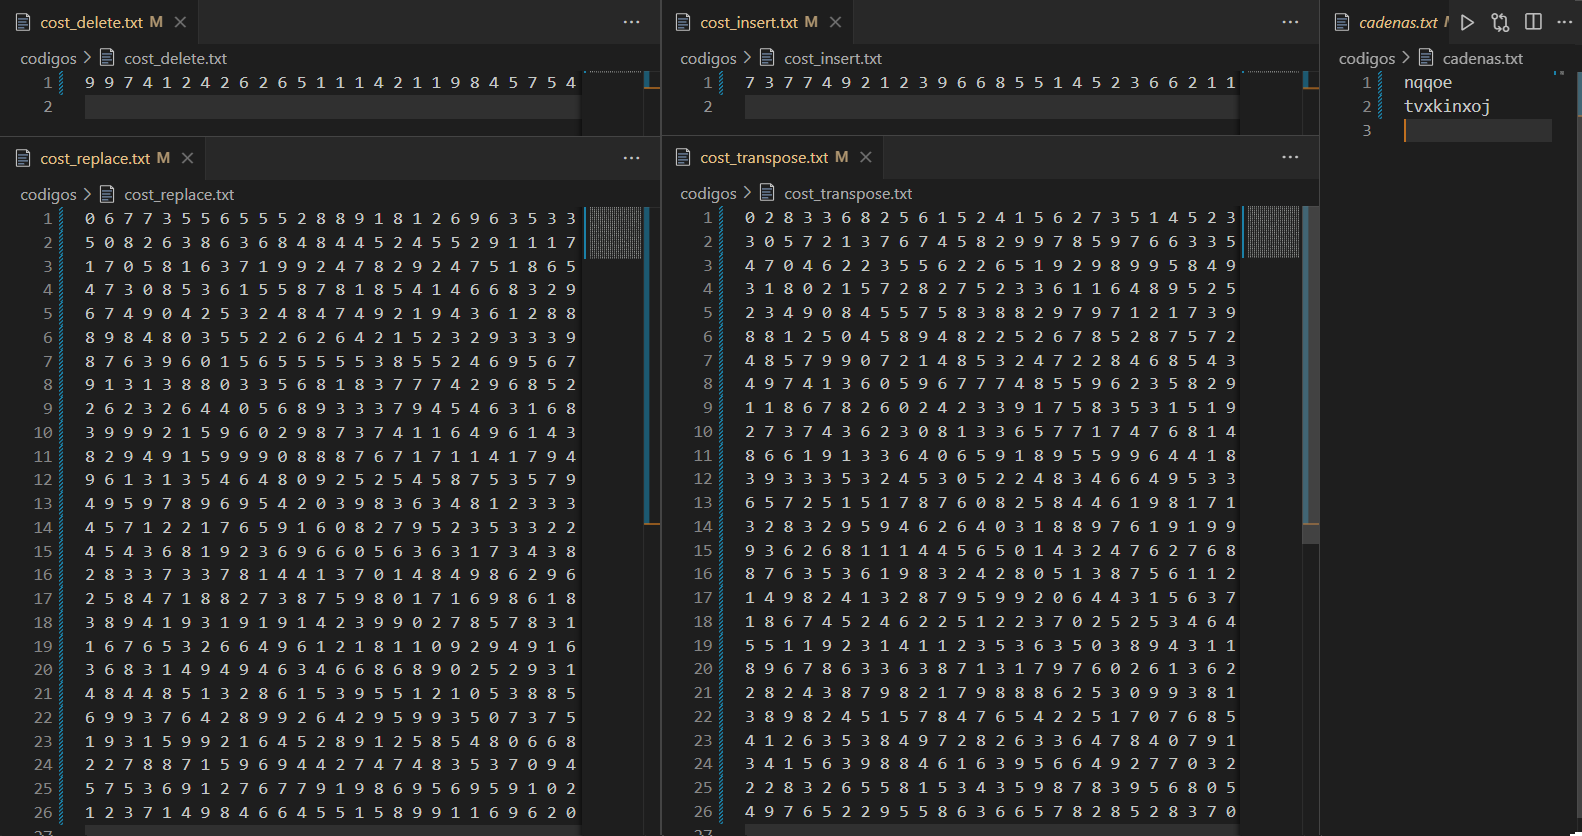
\includegraphics[width=0.6\textwidth]{./images/Casos4.png}
  \caption{Tablas de costo y Cadenas para el Caso con Cadenas Asimétricas}
  \label{fig:imagen4}
\end{figure}

\begin{figure}[ht]
  \centering
  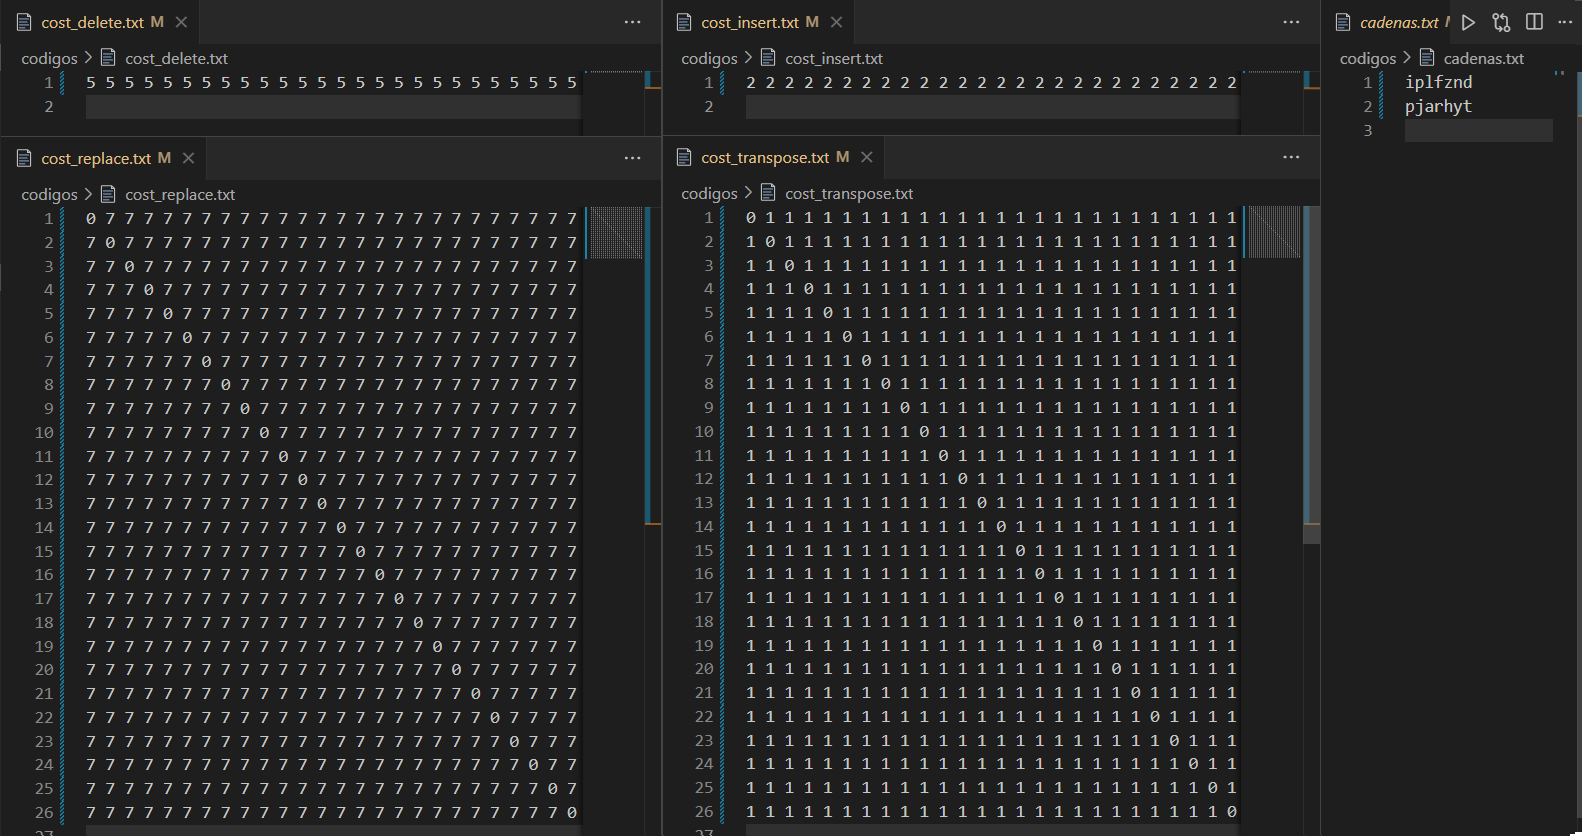
\includegraphics[width=0.6\textwidth]{./images/Casos5.png}
  \caption{Tablas de Costo y Cadenas para el Caso con Matrices de Iguales Valores}
  \label{fig:imagen5}
\end{figure}
\newpage

\begin{figure}[h!]
    \centering
    \begin{minipage}{0.47\textwidth}
        \centering
        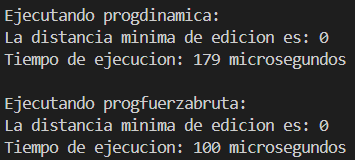
\includegraphics[width=\linewidth]{./images/Resultados1.png}
        \caption{Resultados Caso de Cadenas Vacías}
        \label{fig:imagen6}
    \end{minipage}
    \hfill
    \begin{minipage}{0.47\textwidth}
        \centering
        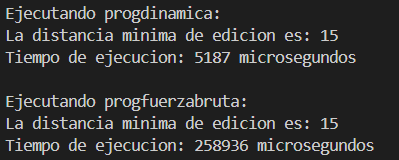
\includegraphics[width=\linewidth]{./images/Resultados2.png}
        \caption{Resultados Caso Caracteres Repetidos}
        \label{fig:imagen7}
    \end{minipage}

    \vspace{1em}

    \begin{minipage}{0.47\textwidth}
        \centering
        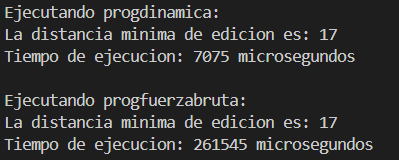
\includegraphics[width=\linewidth]{./images/Resultados3.png}
        \caption{Resultados Caso Cadenas Simétricas}
        \label{fig:imagen8}
    \end{minipage}
    \hfill
    \begin{minipage}{0.47\textwidth}
        \centering
        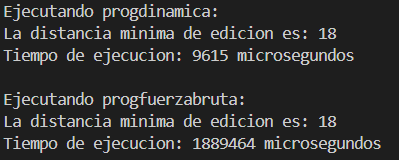
\includegraphics[width=\linewidth]{./images/Resultados4.png} 
        \caption{Resultados Caso Cadenas Asimétricas}
        \label{fig:imagen9}
    \end{minipage}

    \vspace{1em}

    \centering
    \begin{minipage}{0.5\textwidth}
        \centering
        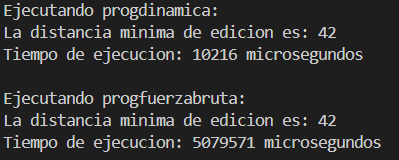
\includegraphics[width=\linewidth]{./images/Resultados5.png} 
        \caption{Resultados Caso Matrices Valores Iguales}
        \label{fig:imagen10}
    \end{minipage}
\end{figure}
\printbibliography

\end{document}
